% 请确保文件编码为utf-8,使用XeLaTex进行编译,或者通过overleaf进行编译

\documentclass[answers]{exam}  % 使用此行带有作答模块
% \documentclass{exam} % 使用此行只显示题目

\usepackage{xeCJK}
\usepackage{zhnumber}
\usepackage{graphicx}
\usepackage{hyperref}
\usepackage{amsmath}
\usepackage{booktabs}
\usepackage{enumerate}
\usepackage{amssymb}
\usepackage{graphicx}
\usepackage{float}

\pagestyle{headandfoot}
\firstpageheadrule
\firstpageheader{南京大学}{机器学习导论}{习题一}
\runningheader{南京大学}
{机器学习导论}
{习题一}
\runningheadrule
\firstpagefooter{}{第\thepage\ 页(共\numpages 页)}{}
\runningfooter{}{第\thepage\ 页(共\numpages 页)}{}


\setlength\linefillheight{.5in}

\renewcommand{\solutiontitle}{\noindent\textbf{解:}\par\noindent}

\renewcommand{\thequestion}{\zhnum{question}}
\renewcommand{\questionlabel}{\thequestion .}
\renewcommand{\thepartno}{\arabic{partno}}
\renewcommand{\partlabel}{\thepartno .}


\begin{document}
\Large
\noindent
% 姓名学号
姓名:麻超 \\
学号:201300066 \\
\begin{questions}
    \question [30] \textbf{概率论基础}

    教材附录C介绍了常见的概率分布.
    给定随机变量$X$的概率密度函数如下,
    \begin{equation}
        f_X(x) =
        \begin{cases}
            \frac{1}{4} & 0<x<1;            \\
            \frac{3}{8} & 3<x<5;            \\
            0           & \mbox{otherwise.}
        \end{cases}
    \end{equation}

    \begin{enumerate}
        \item  请计算随机变量$X$的累积分布函数$F_X(x)$;
        \item  随机变量$Y$定义为$Y = 1/X$, 求随机变量$Y$对应的概率密度函数$f_Y(y)$;
        \item  试证明, 对于非负随机变量$Z$, 如下两种计算期望的公式是等价的.
              \begin{equation}
                  \label{ch1-eq-expect-1}
                  \mathbb{E}[Z] = \int_{z=0}^{\infty}zf(z) \mathrm{d} z.
              \end{equation}

              \begin{equation}
                  \label{ch1-eq-expect-2}
                  \mathbb{E}[Z] = \int_{z=0}^{\infty}\Pr[Z\geq z] \mathrm{d} z.
              \end{equation}
              同时, 请分别利用上述两种期望公式计算随机变量$X$和$Y$的期望, 验证你的结论.
    \end{enumerate}
    \begin{solution}
        % 请在此处作答
        1.
        当$x\leq 0$时,$F_X(x)=0.$

        当$x>5$时,$F_X(x)=1.$

        当$0<x<1$时,$F_X(x)=\int_{-\infty}^x f(x)\ dx=\int_{-\infty}^0 0\ dx+\int_{0}^x \frac{1}{4} \ dx=\frac{1}{4} x.$

        当$1\leq x\leq 3$时,$F_X(x)=\int_{-\infty}^1 \frac{1}{4} \ dx=\frac{1}{4} $

        当$3<x<5$时,$F_X(x)=\int_{-\infty}^x f(x)\ dx=\int_{-\infty}^0 0\ dx+\int_{0}^1 \frac{1}{4} \ dx+\int_{1}^3 0\ dx+\int_{3}^x \frac{3}{8} \ dx= \frac{3}{8} x-\frac{7}{8} .$

        所以所求分布函数是
        \begin{align*}
            F_X(x)=
            \begin{cases}
                0,                         & \ x\leq 0         \\
                \frac{1}{4} x ,            & \ 0< x< 1         \\
                \frac{1}{4},               & \ 1\leq  x\leq 3  \\
                \frac{3}{8} x-\frac{7}{8}, & \ 3<x<5           \\
                1,                         & \text{} x\geq 5 .
            \end{cases}
        \end{align*}

        2.
        $Y$的取值范围为$(0,\infty)$,先求$Y$的分布函数,由于$X>0$,所以$Y>0$.故当$y\leq 0$时,$F_Y(y)=0,f_Y(y)=0.$当$y>0$时,

        $F_Y(y)=P(\frac{1}{X}\leq y )=P(X\geq \frac{1}{y} )=1-P(X< \frac{1}{y} )=1-F_X(\frac{1}{y} )$

        $f_Y(y)=-f_X(\frac{1}{y} )(-\frac{1}{y^2} )=f_X(\frac{1}{y} )(\frac{1}{y^2} )$

        所以所求概率密度函数为

        \begin{align*}
            f_Y(y)=
            \begin{cases}
                \frac{1}{4} \frac{1}{y^2} , & \ y>1                        \\
                \frac{3}{8} \frac{1}{y^2} , & \ \frac{1}{5} <y<\frac{1}{3} \\
                0,                          & \ otherwise
            \end{cases}
        \end{align*}
        3.随机变量Z的概率密度为$f(z)$,有:
        \begin{align*}
            \mathbb E(Z) & =\int_0^\infty zf(z)dz          \\
                         & =\int_0^\infty\int_0^z dxf(z)dz
        \end{align*}
        交换积分次序得到
        \begin{align*}
            \mathbb E(Z) & =\int_0^\infty\int_x^\infty f(z)dzdx \\
                         & =\int_0^\infty P(Z\geq x)dx
        \end{align*}
        由于积分与积分符号无关,所以有

        $\mathbb E(Z)=\int_0^\infty P(Z\geq z)dz$

        得证.

        对于随机变量X:第一种方法:
        \begin{align*}
            \mathbb E[X]=\int_0^\infty xf_X(x)\ dx=\int_0^1\frac{1}{4} x\ dx+\int_3^5 \frac{3}{8} x\ dx=\frac{25}{8}
        \end{align*}

        第二种方法:
        \begin{align*}
            \mathbb E[X] & =\int_0^\infty Pr[X\geq x]\ dx \\&=\int_0^\infty(1-F_X(x))\ dx\\&=\int_0^1(1-\frac{x}{4} )\ dx+\int_1^3 \frac{3}{4} \ dx+\int_3^5(\frac{15}{8} -\frac{3}{8}x) \ dx \\& =\frac{25}{8}
        \end{align*}

        对于随机变量Y:第一种方法:
        \begin{align*}
            \mathbb E[Y] & =\int_0^\infty yf_Y(y)\ dy \\&=\int_{\frac{1}{5} }^{\frac{1}{3} }\frac{3}{8} \frac{1}{y} \ dy+\int_1^\infty \frac{1}{4} \frac{1}{y} \ dy\\&=+\infty
        \end{align*}

        第二种方法:
        \begin{align*}
            \mathbb E[Y] & =\int_0^\infty Pr[Y\geq y]\ dy \\&=\int_0^\infty(1-F_Y(y))\ dy\\&=\int_{\frac{1}{5} }^{\frac{1}{3} }(\frac{3}{8y} -\frac{7}{8} )\ dy+\int_{\frac{1}{3} }^1 \frac{1}{4} \ dy+\int_1^\infty(\frac{1}{4y}) \ dy \\& =+\infty
        \end{align*}
    \end{solution}


    \question [40] \textbf{评估方法}

    教材2.2.3节描述了自助法~(bootstrapping), 下面考虑将自助法用于对统计量估计这一场景, 并对自助法做进一步分析.
    考虑$m$个从分布$p(x)$中独立同分布抽取的(互不相等的)观测值$x_1, x_2, \ldots, x_m$, $p(x)$的均值为$\mu$, 方差为$\sigma^2$. 通过$m$个样本, 可使用如下方式估计分布的均值
    \begin{equation}
        \bar{x}_m = \frac{1}{m} \sum_{i=1}^{m} x_{i}\;,\label{ch2_eq:estimate_mean}
    \end{equation}
    和方差
    \begin{equation}
        \bar{\sigma}^2_m=\frac{1}{m-1} \sum_{i=1}^{m}\left(x_{i}-\bar{x}_m\right)^{2}\label{ch2_eq:estimate_variance}
    \end{equation}
    设$x^*_1, x^*_2, \ldots, x^*_m$为通过自助法采样得到的结果, 且
    \begin{equation}
        \bar{x}^*_m = \frac{1}{m} \sum_{i=1}^{m} x^*_{i}\;,
    \end{equation}
    \begin{enumerate}
        \item 请证明$\mathbb E[\bar{x}_m] = \mu$且$\mathbb E[\bar{\sigma}^2_m] = \sigma^2$;
        \item 计算$var[\bar{x}_m]$;
        \item 计算$\mathbb E[\bar{x}^*_m \mid x_1, \ldots, x_m]$和$var[\bar{x}^*_m \mid x_1, \ldots, x_m]$;
        \item 计算$\mathbb E[\bar{x}^*_m]$和$var[\bar{x}^*_m]$;
        \item 针对上述证明分析自助法和交叉验证法的不同.
    \end{enumerate}

    \begin{solution}
        %请在此处作答
        1.
        \begin{align*}
            \mathbb E[\bar{x}_m]        & =\mathbb E[\frac{1}{m} \sum_{i=1}^{m}x_i]                  \\&=\frac{1}{m} \mathbb E[\sum_{i=1}^{m}x_i]\\&=\frac{1}{m} m\mu=\mu\\
            \mathbb E[\bar{\sigma}^2_m] & =\frac{1}{m-1} \mathbb E[\sum_{i=1}^{m}(x_i-\bar{x}_m)^2]  \\&=\frac{1}{m-1} \mathbb E[\sum_{i=1}^{m}x_i^2+m\bar{x}_m^2-2\sum_{i=1}^{m}x_i\bar{x}_m]\\&=\frac{1}{m-1}\mathbb E[\sum_{i=1}^{m}x_i^2-m\bar{x}_m^2]\\
            \because var[x]             & =\mathbb E[x^2]-\mathbb E^2[x]                             \\
            \therefore \mathbb E(x_i^2) & =\mu^2+\sigma^2                                            \\
            \mathbb E(x_m^2)            & =var(\bar{x}_m)+\mathbb E^2(\bar{x}_m)                     \\
                                        & \text{由第二问的$var(\bar{x}_m^2)$可以得到}                \\
            \mathbb E(\bar{x}_m^2)      & =\frac{\sigma^2}{m} +\mu^2                                 \\
            \mathbb E(\bar{\sigma}_m^2) & =\frac{1}{m-1} (m\mu^2+m\sigma^2-\sigma^2-m\mu^2)=\sigma^2
        \end{align*}

        2.
        \begin{align*}
            var(\bar{x}_m)=var(\frac{1}{m} \sum_{i=1}^{m}x_i)=\frac{1}{m^2} var(\sum_{i=1}^{m}x_i)=\frac{\sigma^2}{m}
        \end{align*}

        3.
        由独立同分布可得:
        \begin{align*}
            \mathbb E[\bar{x}^*_m \mid x_1, \ldots, x_m] & =\frac{1}{m} \sum_{i=1}^{m}\mathbb E[x_i^*]=\bar{x}_m              \\
            var[\bar{x}^*_m \mid x_1, \ldots, x_m]       & = var[\frac{1}{m} \sum_{i=1}^{m}\bar{x}^*_i \mid x_1, \ldots, x_m] \\&=\frac{1}{m^2}var[\sum_{i=1}^{m}\bar{x}^*_i \mid x_1, \ldots, x_m] \\&
            =\frac{1}{m^2} \sum_{i=1}^{m}var[\bar{x}^*_i \mid x_1, \ldots, x_m]                                               \\&=\frac{1}{m^2} \cdot m\cdot \frac{m-1}{m} \cdot \bar{\sigma}_m^2\\&=\frac{m-1}{m^2} \bar{\sigma}_m^2
        \end{align*}

        4.\begin{align*}
            \mathbb E[\bar{x}_m^*] & =\mathbb E(\mathbb E[\bar{x}^*_m \mid x_1, \ldots, x_m])=\mathbb E[\bar{x}_m]=\mu                    \\
            var(\bar{x}_m^*)       & =\mathbb E[var[\bar{x}^*_m \mid x_1, \ldots, x_m]]+var[\mathbb E[\bar{x}^*_m \mid x_1, \ldots, x_m]] \\&=\mathbb E[\frac{m-1}{m^2} \bar{\sigma}_m^2]+var[\bar{x}_m]\\&=\frac{m-1}{m^2} \sigma^2+\frac{\sigma^2}{m} \\&=\frac{2m-1}{m^2} \sigma^2
        \end{align*}

        5.交叉验证法从原数据集中分层采样,可以认为交叉验证法得到的训练集,测试集与原数据集分布保持一致,但是自助法为放回采样,不能保证分布保持一致.
    \end{solution}


    \question [30] \textbf{性能度量}

    教材2.3节介绍了机器学习中常用的性能度量. 假设数据集包含8个样例, 其对应的真实标记和学习器的输出值(从大到小排列)如表~\ref{table:roc}所示. 该任务是一个二分类任务, 标记1和0表示真实标记为正例或负例.
    学习器的输出值代表学习器认为该样例是正例的概率.
    \begin{table}[!h]
        \centering
        \caption{样例表} \vspace{2mm}\label{table:roc}
        \begin{tabular}{c|c c c c c c c c c c c}\toprule
            样例         & $x_1$ & $x_2$ & $x_3$ & $x_4$ & $x_5$ & $x_{6}$ & $x_{7}$ & $x_{8}$ \\
            \midrule
            标记         & 1     & 1     & 0     & 1     & 0     & 1       & 0       & 0       \\
            \midrule
            分类器输出值 & 0.81  & 0.74  & 0.62  & 0.55  & 0.44  & 0.35    & 0.25    & 0.21    \\
            \bottomrule
        \end{tabular}
    \end{table}
    \begin{enumerate}
        \item 计算P-R曲线每一个端点的坐标并绘图;
        \item 计算ROC曲线每一个端点的坐标并绘图, 计算AUC;
    \end{enumerate}
    \begin{solution}
        %请在此处作答
        1.

        可以看出,该数据集中正例一共有4个,所以查全率=正例的样本/4,查准率=正例样本/学习器认为是正例的个数,以每个样例对应的分类器输出值为阈值,列出表格如下
        \begin{center}
            \begin{tabular}{|c|c|c|c|c|c|c|}
                \hline
                样例对应分类器输出值 & TP & FP & FN & TN & P    & R    \\
                \hline
                x1                   & 1  & 0  & 3  & 4  & 1.0  & 0.25 \\
                \hline
                x2                   & 2  & 0  & 2  & 4  & 1.0  & 0.5  \\
                \hline
                x3                   & 2  & 1  & 2  & 3  & 0.67 & 0.5  \\
                \hline
                x4                   & 3  & 1  & 1  & 3  & 0.75 & 0.75 \\
                \hline
                x5                   & 3  & 2  & 1  & 2  & 0.6  & 0.75 \\
                \hline
                x6                   & 4  & 2  & 0  & 2  & 0.67 & 1.0  \\
                \hline
                x7                   & 4  & 3  & 0  & 1  & 0.57 & 1.0  \\
                \hline
                x8                   & 4  & 4  & 0  & 0  & 0.5  & 1.0  \\
                \hline
            \end{tabular}
        \end{center}
        绘图如下:

        \begin{figure}[H]
            \centering
            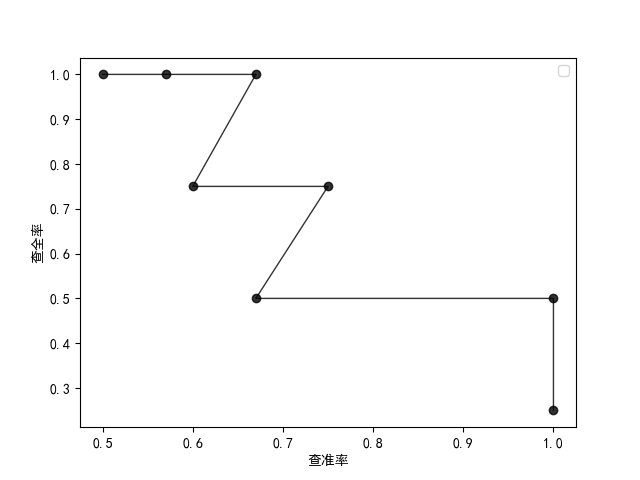
\includegraphics[width=9.5cm,height=9.5cm]{Figure_1.png}
            \caption{P-R曲线}
        \end{figure}


        2.

        根据上一问中得到的结论,可以得到根据划分不同阈值得到的TPR和FPR列表为

        TPR:[0.25,0.5,0.5,0.75,0.75,1.0,1.0,1.0]

        FPR:[0,0,0.25,0.25,0.5,0.5,0.75,1.0]

        绘图如下:

        \begin{figure}[H]
            \centering
            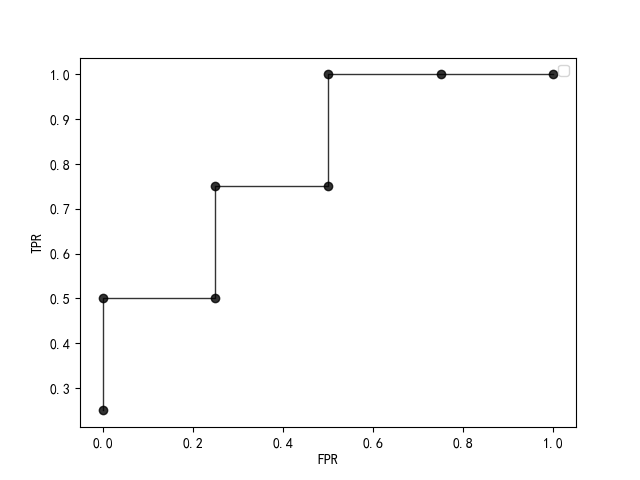
\includegraphics[width=9.5cm,height=9.5cm]{Figure_2.png}
            \caption{ROC曲线}
        \end{figure}
        计算得到:AUC=0.8125
    \end{solution}
\end{questions}


\end{document}